\section{Correlation Puzzle}
As discussed in the paper, there is a low correlation between returns and fundamentals such as dividends, consumption and output, i.e., the correlation puzzle.  Our demand disagreement model can reconcile the low correlation between output growth and stock market returns and it leads to no correlation between   output growth and both the risk-free rate and trading volume. Specifically, Figure \ref{fig:CorrelationPuzzle} shows the correlation between stock market returns and aggregate consumption for the one, five, and ten year horizon as a function of disagreement $\Delta$.  The figure shows that without disagreement, the correlations are close to one. Hence, demand shocks alone are not sufficient to solve the correlation puzzle.  When disagreement $\Delta$ increases, then the correlation decreases at an increasing rate, and thus for reasonable $\Delta$, we get correlations comparable to the ones we see in the data.  

\begin{figure}[H]
\begin{center}
       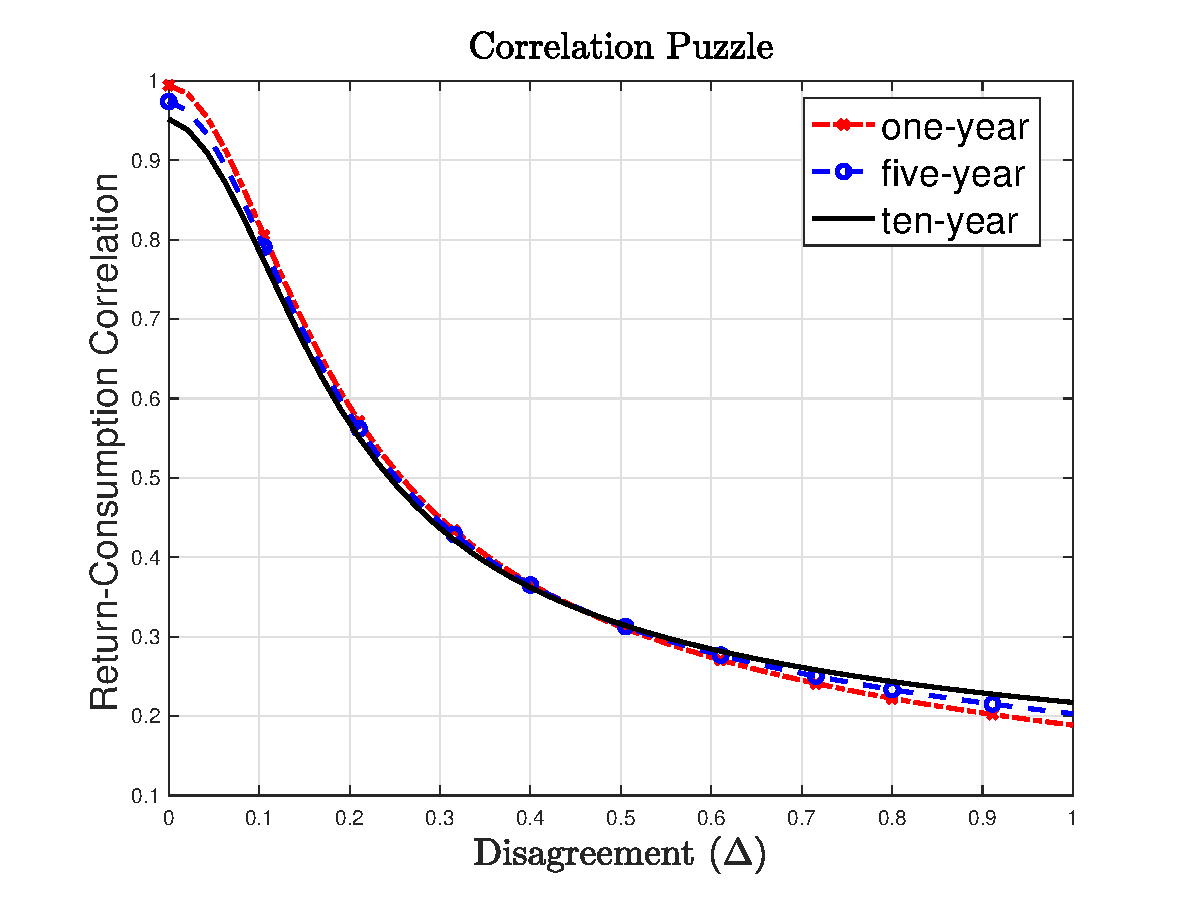
\includegraphics[height=6cm]{figures/CorrelationPuzzle2DEL.eps}  
     \captionsetup{labelformat=andtable}
     \end{center}
\renewcommand\thetable{1}
\caption{\textbf{Correlation puzzle.} \footnotesize{The figure shows the unconditional correlation between stock market returns and aggregate consumption for a one, five and ten year horizon as a function of disagreement $\Delta$. The correlations are based on one million years of monthly observations. In this example the parameters are based on the alternative calibration with $\rho^a = 0.001$ and $\rho^b = 0.05$ }} \label{fig:CorrelationPuzzle} 
\end{figure}

What is the economic intuition for this low correlation in our model? Suppose there are no demand shocks, then the price dividend ratio is constant and stock market returns are perfectly correlated with output shocks. When there are commonly perceived demands shocks, then the price dividend ratio is stochastic but its dynamics are locally deterministic; hence short term correlations between stock market returns and consumption are close to one. The correlation is $0.95$ when measured over ten years and, thus, the indirect effect of the demand shock through the drift of the consumption share is quantitatively small.  The indirect effect is small because heterogeneous time preferences only lead to different consumption-savings rates.   In contrast, when agents have different beliefs about demand shocks, they engage in speculative trade, thus changing their consumption-saving rates and portfolio compositions. Demand shocks, which are by assumption independent of output shocks, lead to shocks to the price-dividend ratio, the risk free rate, the volatility and risk premium of the stock market, and trading volume. Hence, demand disagreement breaks the tight link between shocks to output growth and stock market returns and solves the correlation puzzle.   Similar to the risk-free rate, disagreement and the resulting trade in the stock market is purely driven by demand shocks and, hence, the correlation between macroeconomic fundamentals and both the risk-free rate and trading volume, which is also low in the data, is by construction zero.\footnote{It is straightforward to increases this correlation by adding disagreement about output growth.} 

From the above discussion it is clear that in our model the correlation puzzle and the disagreement correlation puzzle are closely related -- all disagreement in asset prices are due to demand disagreement  and without demand disagreement the model cannot generate sufficient disconnect between asset prices and macroeconomic fundamentals to replicate the correlation puzzle. 
